\documentclass[table, 12pt]{article} % \documentclass{} is the first command in any LaTeX code.  It is used to define what kind of document you are creating such as an article or a book, and begins the document preamble

\usepackage[T1]{fontenc}
\usepackage[utf8]{inputenc}
\usepackage[english]{babel}
\usepackage{graphicx}
\usepackage{titlesec}
\usepackage{hyperref}
\usepackage[usenames,dvipsnames]{xcolor}
\usepackage{float}
\usepackage[export]{adjustbox}
\usepackage{longtable}
\usepackage{listings}
%\usepackage{alloy}



% The preamble ends with the command \begin{document}
\begin{document} % All begin commands must be paired with an end command somewhere
    
    \begin{titlepage}
        \centering
        {\scshape\large AY 2022/2023 \par}
        \vfill
        
\includegraphics[width=200pt]{assets/logo_polimi}\par\vspace{1cm}
        \vspace{0.5cm}
        {\huge\bfseries RASD\@: Requirement Analysis
            and Specification Document \par}
        \vspace{1cm}
        {\large {Marcello De Salvo\quad Riccardo Grossoni \par Francesco Dubini}\par}
        \vfill
        {\large Professor\par
            Elisabetta \textsc{Di Nitto}}
        \vfill
        {\large \textbf{Version 0.1}\\ \today \par}
    \end{titlepage}
    
    \thispagestyle{plain}
    \pagenumbering{gobble}

    % Blank page
    \mbox{}

    % Table of content page
    \newpage
    \pagenumbering{roman}
    \tableofcontents

    % Start of the document
    \newpage
    \pagenumbering{arabic}

    \section{Introduction}
        \emph{Electric mobility} (e-Mobility) is a way to reduce the carbon footprint caused by motorized vehicles in urban and sub-urban areas.\\
        % One way to do so while using an electric vehicle is to fit and optimize the charging process into our daily schedule
        Comfortably knowing how to fit the charging process into one's daily schedule is a fundamental step towards that goal.
        
    \subsection{Purpose} %goals of the project

        %One of the biggest drawbacks of electric vehicles is the toll the charging process takes in terms of time. So on and so forth
         
        In the last 3 years the number of electric vehicles has doubled and, with the proposed european legislation on banning diesel fuel by 2035, the future seems to be full-electric. This rapid change requires a better and more efficient infrastructure to serve this ever increasing demand.

        %In these years the number of electric vehicles has been on the rise and, as it is expcted to be quadrupled by 2050, a better working infrastructure for them is needed.
        
        %Electric vehicles will quadruple in the next 5 years. As of now, having to charge your car in the middle of the day can prove to be a very daunting task

        \emph{eMall} (e-Mobility for all) aims to ease the charging process for the users through the \emph{e-Mobility Service Provider's} (eMSP) platform,
        providing all the needed end-users' services and by actively communicating with multiple \emph{Charging Point Operators'} (CPOs) \emph{Management Systems} (CPMS).
        The eMall platform will also provide a dashboard for the \emph{Charging Point Operators' workers}(CPOW) to change some settings that can also be done automatically by the CPMS.

    \subsubsection{Goals}
        \newcounter{goalCtr}
        \underline{User goals}
        \begin{itemize}
            \item  \textbf{(\stepcounter{goalCtr}G\arabic{goalCtr}) Know about the charging stations nearby, including their cost and any special offer they have.}
            \item  \textbf{(\stepcounter{goalCtr}G\arabic{goalCtr}) Book a charge in a specific charging station for a certain timeframe.}\\ description
            \item  \textbf{(\stepcounter{goalCtr}G\arabic{goalCtr}) Start the charging process at a certain station.}
            \item  \textbf{(\stepcounter{goalCtr}G\arabic{goalCtr}) Pay for the obtained service.}
        \end{itemize}
        
        \newpage
        \underline{eMSP goals}
        \begin{itemize}
            \item  \textbf{(\stepcounter{goalCtr}G\arabic{goalCtr}) Be able to communicate with multiple CPMS.}
            \item  \textbf{(\stepcounter{goalCtr}G\arabic{goalCtr}) Suggest the user convenient charging timeframes based on his upcoming schedule.}
            \item  \textbf{(\stepcounter{goalCtr}G\arabic{goalCtr}) Notify the user when the charging process is finished.}
        \end{itemize}
        
        \underline{CPMS goals}
        \begin{itemize}
            \item  \textbf{(\stepcounter{goalCtr}G\arabic{goalCtr}) Be able to communicate with multiple eMSPs.}
            \item  \textbf{(\stepcounter{goalCtr}G\arabic{goalCtr}) Be able to communicate with at least one DSO.}
            \item  \textbf{(\stepcounter{goalCtr}G\arabic{goalCtr}) Communicate the location and “external” status of a charging station.}
            \item  \textbf{(\stepcounter{goalCtr}G\arabic{goalCtr}) Know the “internal” status of a charging station .}
            \item  \textbf{(\stepcounter{goalCtr}G\arabic{goalCtr}) Start charging a vehicle according to the amount of power supplied by the socket, and monitor the charging process to infer when the battery is full.}
            \item  \textbf{(\stepcounter{goalCtr}G\arabic{goalCtr}) Acquire from the DSOs information about the current price of energy.}
            \item  \textbf{(\stepcounter{goalCtr}G\arabic{goalCtr}) Decide from which DSO to acquire energy (if more than one is available).}
            \item  \textbf{(\stepcounter{goalCtr}G\arabic{goalCtr}) Dynamically decide where to get energy for charging (station battery, DSO, or a mix according to availability and cost).}
        \end{itemize}

        \underline{CPOW goals}
        \begin{itemize}
            \item  \textbf{(\stepcounter{goalCtr}G\arabic{goalCtr}) Change the source of energy between batteries and grid.}
            \item  \textbf{(\stepcounter{goalCtr}G\arabic{goalCtr}) Insert special and limited offers.}
            \item  \textbf{(\stepcounter{goalCtr}G\arabic{goalCtr}) Change the price of a charging station.}
        \end{itemize}

    \newpage
    \subsection{Scope} %analysis of the world and shared phenomena
    %ADD: basic service and advanced functionalities
    \subsubsection*{Shared Phenomena}
        \newcounter{sharedP}
        \rowcolors{2}{red!25}{}
        \begin{center}
        \begin{tabular}{|c|p{0.70\textwidth}|c|}
            \hline
            \textbf{ID} & \textbf{Phenomenom} &  \textbf{Controller}\\\hline\hline
            \stepcounter{sharedP}
            S\arabic{sharedP} & User registers through the application & World \\\hline
            \stepcounter{sharedP}
            S\arabic{sharedP} & User logs into the application & World \\\hline %might remove this
            \stepcounter{sharedP}
            S\arabic{sharedP} & User gets notified by the system about the status of the charge & Machine \\\hline
            \stepcounter{sharedP}
            S\arabic{sharedP} & User is suggested by the system to go and charge the vehicle, depending on the status of the battery, his daily schedule and the charging type & Machine \\\hline
            \stepcounter{sharedP}
            S\arabic{sharedP} & User is presented with special offers made available by some CPOs & Machine\\\hline
            \stepcounter{sharedP}
            S\arabic{sharedP} & The system shows the availability of nearby charging stations &  Machine \\\hline%User checks the availability of charging slots at nearby stations%
            \stepcounter{sharedP}
            S\arabic{sharedP} & User pays the cost of the charge through the application & World \\\hline
            \stepcounter{sharedP}
            S\arabic{sharedP} & CPOW inserts a new discount into the system & World \\\hline
            
            \hline
        \end{tabular}
        \end{center}
    
    \subsubsection*{World Phenomena}
    \newcounter{worldP}
    \begin{center}
        \rowcolors{2}{red!25}{}
        \begin{tabular}{|c|p{0.70\textwidth}|c|}
            \hline
            \textbf{ID} & \textbf{Phenomenom}\\\hline\hline
            \stepcounter{worldP}
            W\arabic{worldP} & Power outage in a station nearby area\\\hline
            \stepcounter{worldP}
            W\arabic{worldP} & Physical problem in the charging station\\\hline
            \stepcounter{worldP}
            W\arabic{worldP} & Physical problem in the electric vehicle\\\hline
            \stepcounter{worldP}
            W\arabic{worldP} & Unexpected changes in the user daily schedule\\\hline
            \stepcounter{worldP}
            W\arabic{worldP} & Person other than the user is driving the car\\\hline
            \hline
        \end{tabular}
    \end{center}
    
    \newpage
    \subsection{Definitions, acronyms, abbreviations}
    \subsubsection*{Definitions}
        \begin{itemize}
            \item \textbf{User}: any electric car owner.
            \item \textbf{e-Mobility Service Providers}: company offering an electric vehicle charging service to drivers by providing access to multiple charging points around a geographic area.
            \item \textbf{Charging Point Operator}: charging point stations owner.
            \item \textbf{Charge Point Management System}: charging Point Operator's IT infrastructure. Handles the acquisition of energy from external Distribution System Operators and distributes it to the connected vehicles. It can also makes automatic decisions, such as the amount of energy to be used for each connected vehicle.
            \item \textbf{Distribution System Operator}: entity responsible for distributing and managing energy from the generation sources to the final consumers.
            \item \textbf{Open Charge Point Interface}: open protocol used for connections between charge station operators and service providers.
            \item \textbf{Open Charge Point Protocol}: open protocol used for connections between charge stations and their charge point management system.
            \item \textbf{DIN SPEC 70121}: Standard for digital communication between a charging station and an electric vehicle.
            \item \textbf{ISO 15118}: Alternative standard for digital communication between a charging station and an electric vehicle.
        \end{itemize}

    \subsubsection*{Acronyms}
        \begin{itemize}
            \item \textbf{EV}: Electric vehicle
            \item \textbf{eMSP}: e-Mobility Service Providers
            \item \textbf{CPO}: Charging Point Operator
            \item \textbf{CPMS}: Charge Point Management System
            \item \textbf{OCPI}: Open Charge Point Interface
            \item \textbf{OCPP}: Open Charge Point Protocol
            \item \textbf{DSO}: (3rd party) Distribution System Operator
            \item \textbf{API}: Application Programming Interface
            \item \textbf{UML}: Unified Modeling Language
            \item \textbf{CPOW}: Charging Point Operator Worker
            \item \textbf{BESS}: Battery Energy Storage System
        \end{itemize}

    \newpage
    \subsection{Revision history}
        \begin{itemize}
            \item Version 0.1: Setup
            \begin{itemize}
                \item[--] Created first layout
            \end{itemize}
        \end{itemize}

    \subsection{Reference documents}
        \begin{itemize}
            \item Specification document: "Assignment RDD AY 2022-2023"
            \item Alloy documentation: https://alloytools.org/documentation.html
            \item Data on number of electric vehicles: https://www.iea.org/data-and-statistics/charts/global-electric-car-stock-2010-2021
        \end{itemize}
    
    \subsection{Document structure}
        \begin{itemize}
            \item \textbf{Section 1}: introduces the problem, describes every goal of the project and gives an analysis of the world and shared phenomena.
            \item \textbf{Section 2}: gives an overall description of the project and all the interactions that will occur between the system and the final users, including a list of possible scenarios and a description of all the actors involved. It provides also an UML class diagram that will be used as a reference point for the developers.
            \item \textbf{Section 3}: includes all the project's requirements and an in-depth description everything presented in Section 2.
            \item \textbf{Section 4}: shows the Alloy model defined for this project.
        \end{itemize}

    \newpage



    

    \section{Overall Description}

    \subsection{Product perspective}
    In this section we mainly describe some typical scenarios, all the \textit{Product Functions (\ref{product_functions})} offered by the eMall system and the\textit{UML(\ref{class_diagram})} class-diagram.

        \subsubsection{Scenarios}
        \label{scenarios}
            \begin{enumerate}
            
            \item Mister Fontana has just bought an electric vehicle and wants to create an account for the application.  
            \begin{itemize}
                \item He opens the web app and clicks the "Sign Up" button
                \item He inserts all the required information in the mandatory fields and presses the "Confirm" button
                \item The system verifies that the mail has not been used before. After passing the verification a confirmation e-mail is sent to mister Fontana's mailbox
                \item He checks his mailbox to see if he received the confimation e-mail
            \end{itemize}
                
            \item Mister Brambilla is about to finish a meeting and is about to have a 2 hour break. eMall detects that he's about to go on break, and it sends him an e-mail suggesting him to charge his car
            \begin{itemize}
                \item He receives an e-mail suggesting him to charge his car 
                \item He logs on the eMall webapp
                \item The eMall webapp suggests the closest chargers and the ones with eventual discounts
                \item Brambilla selects his preferred charging station and books it
                \item eMall prompts a link to help Brambilla get there
                \item Brambilla opens the link and heads there
            \end{itemize}

            \item Mister Fontana is on vacation and since he's new to the area he wants to know which charging stations are nearby
            \begin{itemize}
                \item He opens the web application and logs-In
                \item He navigates to the interactive map section
                \item He clicks the "current position" button
                \item He gets notified by the web application that his GPS position is not turned on
                \item He turns on the GPS and then searches all the nearby stations by simply clicking the "current position" button and viewing the map 
                
            \end{itemize}
            
            \item Miss Sala will go to the hairdresser next sunday. She knows that in the parking lot near the hairdresser there's a charging station and she wants to make sure that a spot will be available that day, so she decides to book a spot for that charging station
            \begin{itemize}
                \item She opens the web application and logs-In
                \item She selects the "Book a spot" option
                \item She compiles the requested fields with date, time of arrival and location and selects confirm
                \item The system checks if a charging spot for that date and time is still available, in that case a confirmation message is shown and the booking is saved. If no spot is still available an "unsuccesful booking" message is shown and the booking is aborted
                \item After successfully booking a spot the system sends a mail with a recap of the booking 
                \item Miss Sala after reaching the charging station on the booked timeframe unlocks the booked charging spot via the web app and can start the starting process
            \end{itemize}
            
            \item Mister Ferrari has booked a charging spot for saturday. He realizes that he has lost the keys to his car, and will not make it in time. While he searches for his keys he forgets to delete the reservation.
            \begin{itemize}
                \item The system locks the charging spot while waiting for mister Ferrari
                \item 5 minutes after the booked time, if the reservated user doesn't show up, the charging spot is unlocked and the reservation is cancelled
                \item Other users can now start using the previously reserved charging spot
            \end{itemize}

            \item Mister Rana wants to start the charging process and pay, since he's arrived at the booked station near his office
            \begin{itemize}
                \item He opens the web application and logs-In
                \item He navigates to the "booking list" section
                \item He plugs-in the charging cable to the car 
                \item He selects the right station and clicks the "start charging" button
                \item He's then asked to pay inside the web app and he pays with his credit card
                \item He finally sees that the car has started to charge
                \item When the charging ends he gets notified by the application
            \end{itemize}

            \item Mister Rossi wants to plan his trip to Rome with his electric car. He would also like to save money by selecting the cheapest charging stations along the itinerary.
            \begin{itemize}
                \item He opens the web-application and he logs-In
                \item He plans his trip inside the navigation system or the in-app map
                \item He then sorts the charging stations by the charging price and the special offers
                \item He books the cheaper ones that covers the right amount of distance from each other
            \end{itemize}
            
            \item Mister Lamborghini wants to delete his booked charge since his schedule changed and he can no longer make it there in time.
            \begin{itemize}
                \item He opens the web-application and he logs-In
                \item On the webapp he opens his "bookings list"
                \item He then selects the one he wants to delete and clicks on "cancel booking"
                \item An email of the succesful cancellation is sent and the system deletes the previous reservation
            \end{itemize}
            

            
            \end{enumerate}


        \subsubsection{Class diagram}
        \label{class_diagram}
            In the UML diagram there are described all the main entities in the system.
            We can see that the system is composed by 2 main actors: the \textit{User} and the \textit{CPO}.\\
            The user owns an \textit{E-car} and can book a charging spot, while the charging station is the entity that provides the charging service.\\
            Data regarding the charging stations and the sockets are provided by the CPMS \textit{OCPI API} which is used by the \textit{Booking}, \textit{Charging Process} and \textit{Charging station} entities to retrive or send all the needed information, and that is implemented inside the CPMS subsystem.\\
            There's also an entity for the \textit{Socket} in order to store the information about the socket's status and his price, and another one for the \textit{Offer} that can be applied to all the charging stations owned by the same CPO.\\
            Information about the Users' daily schedule are represented inside the \textit{Calendar Schedule} and the the \textit{Event} entity, that use the \textit{Calendar API} to retrive the user's appointments.\\
            There's also an interface for the \textit{Payment} that can be implemented by different payment methods.
            
            \begin{center}
                \begin{figure}[H]
                    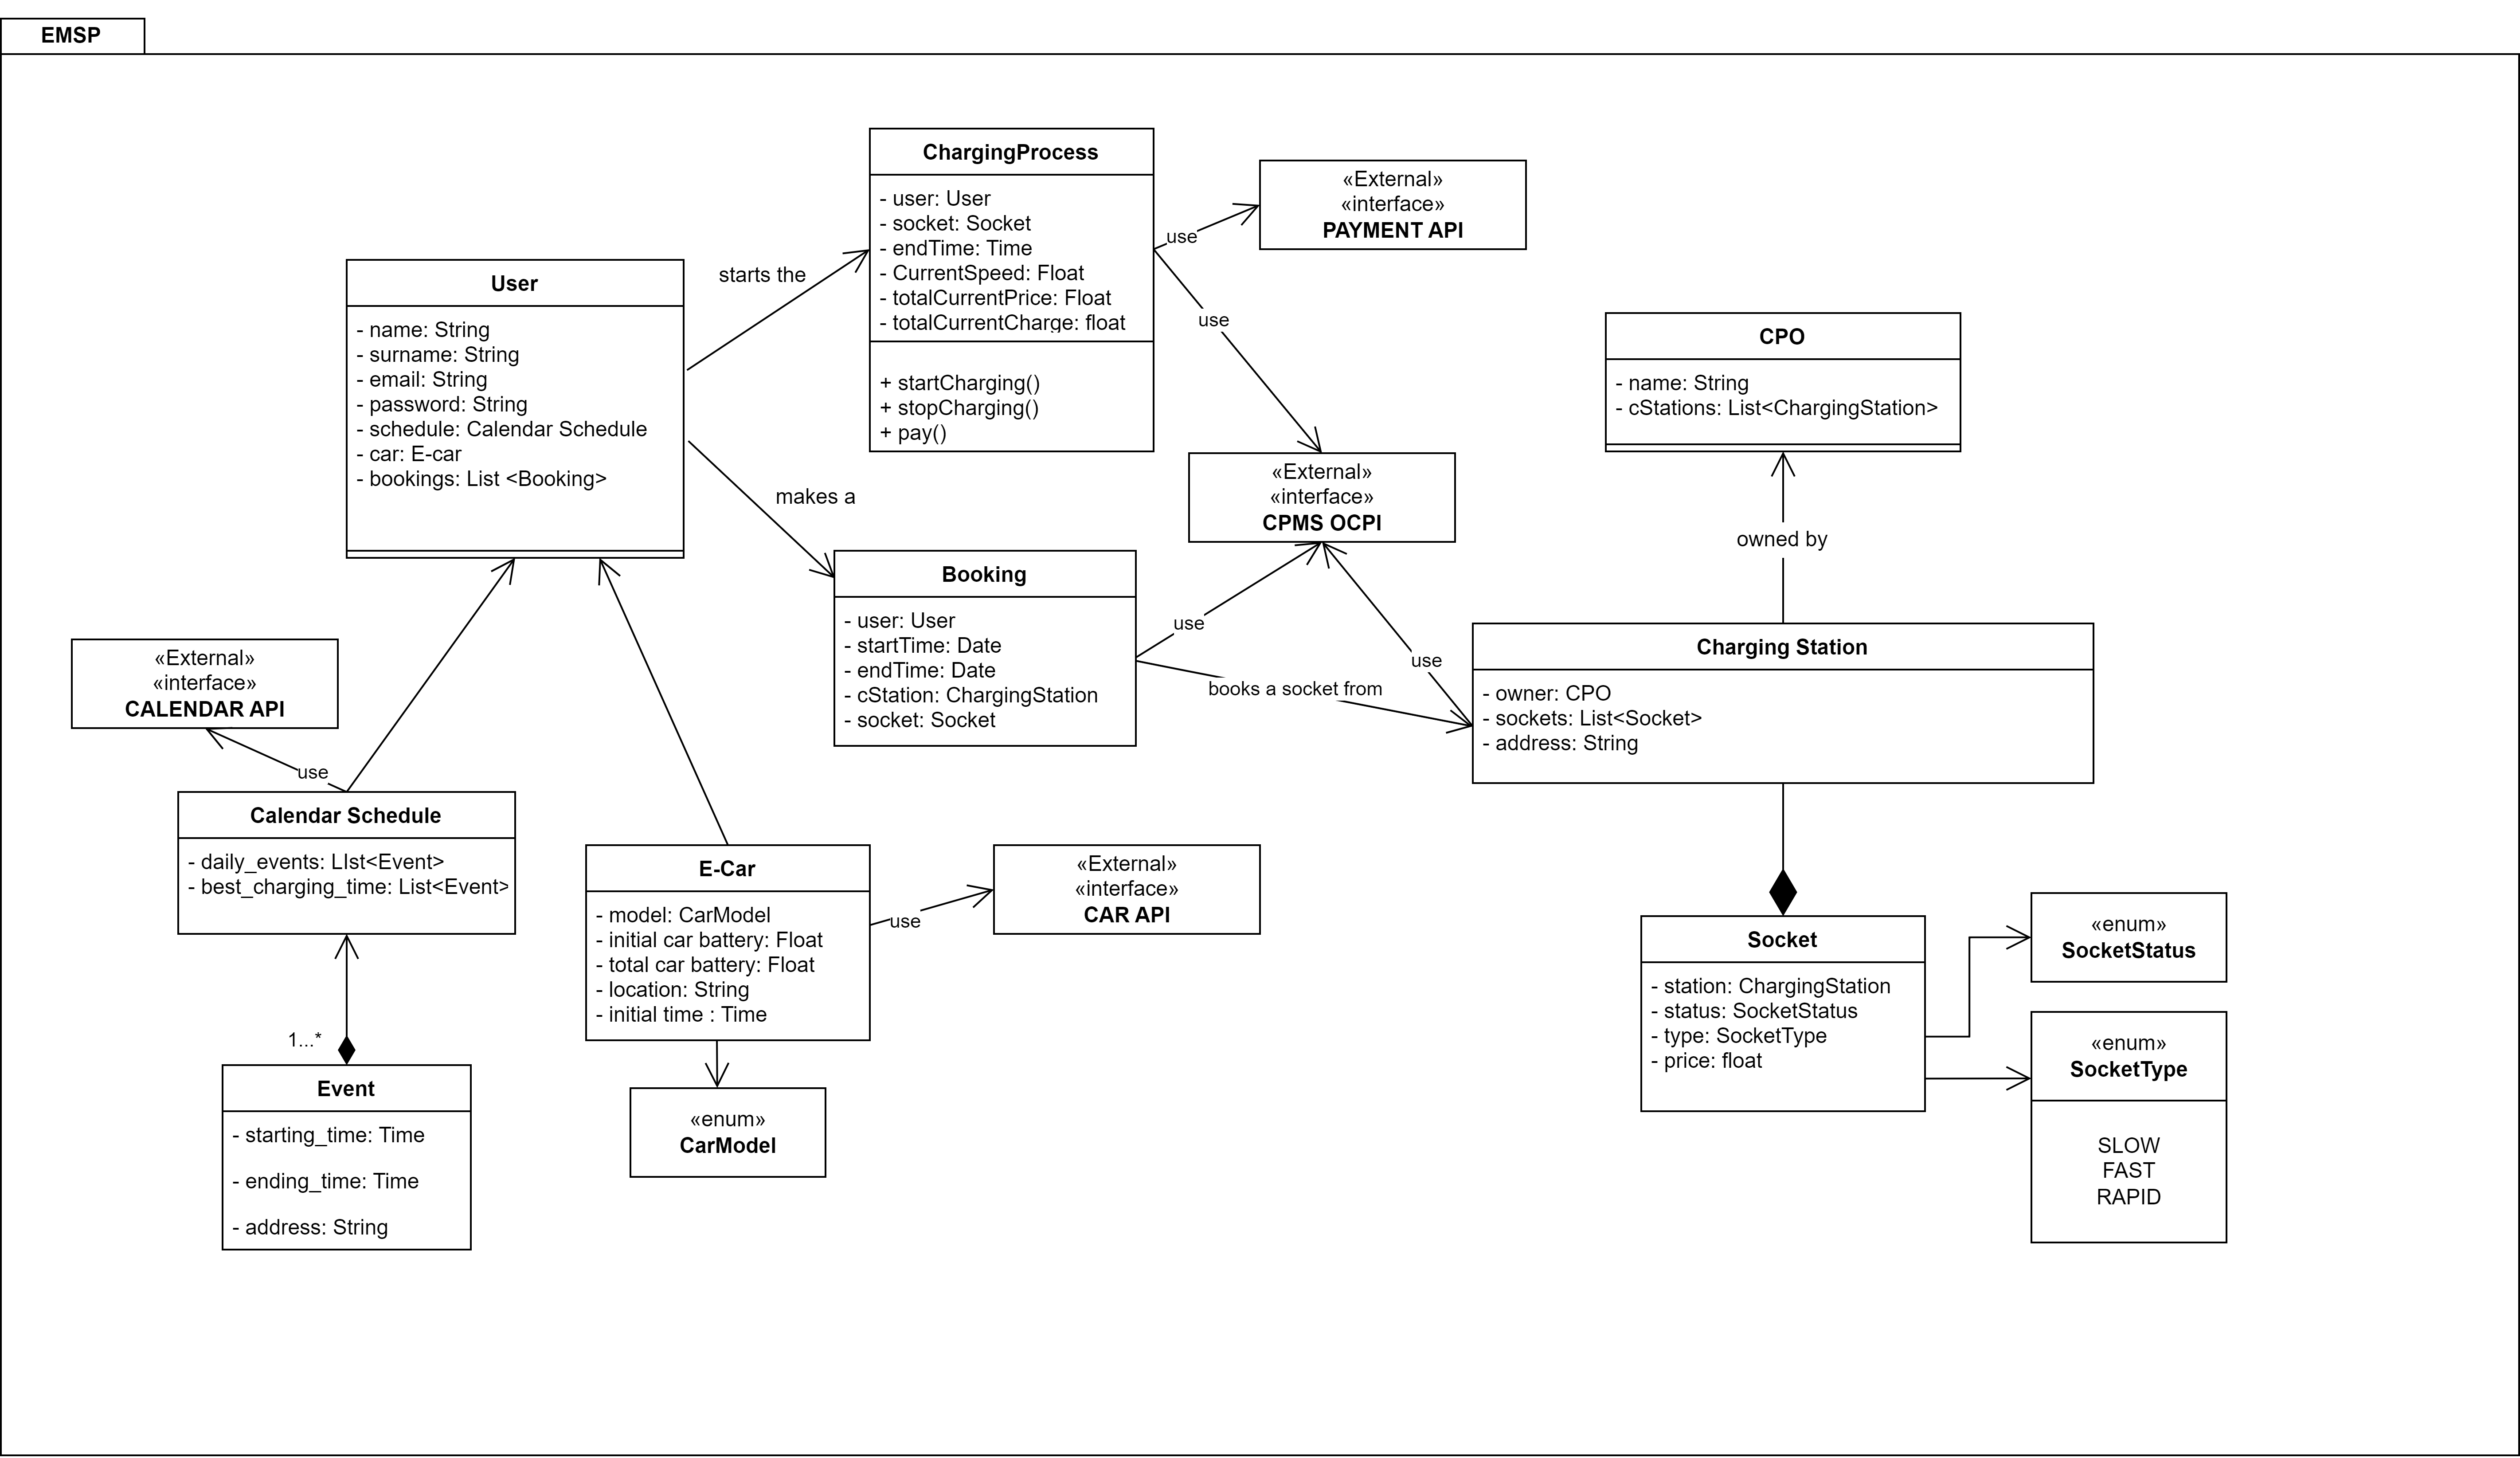
\includegraphics[scale=0.55, center]{assets/UML_EMSP.png}
                    \caption{High-level UML - EMSP Subsystem}
                    \label{fig: UML EMSP}
                \end{figure}
            \end{center}
            \newpage
            \begin{center}
                \begin{figure}[H]
                    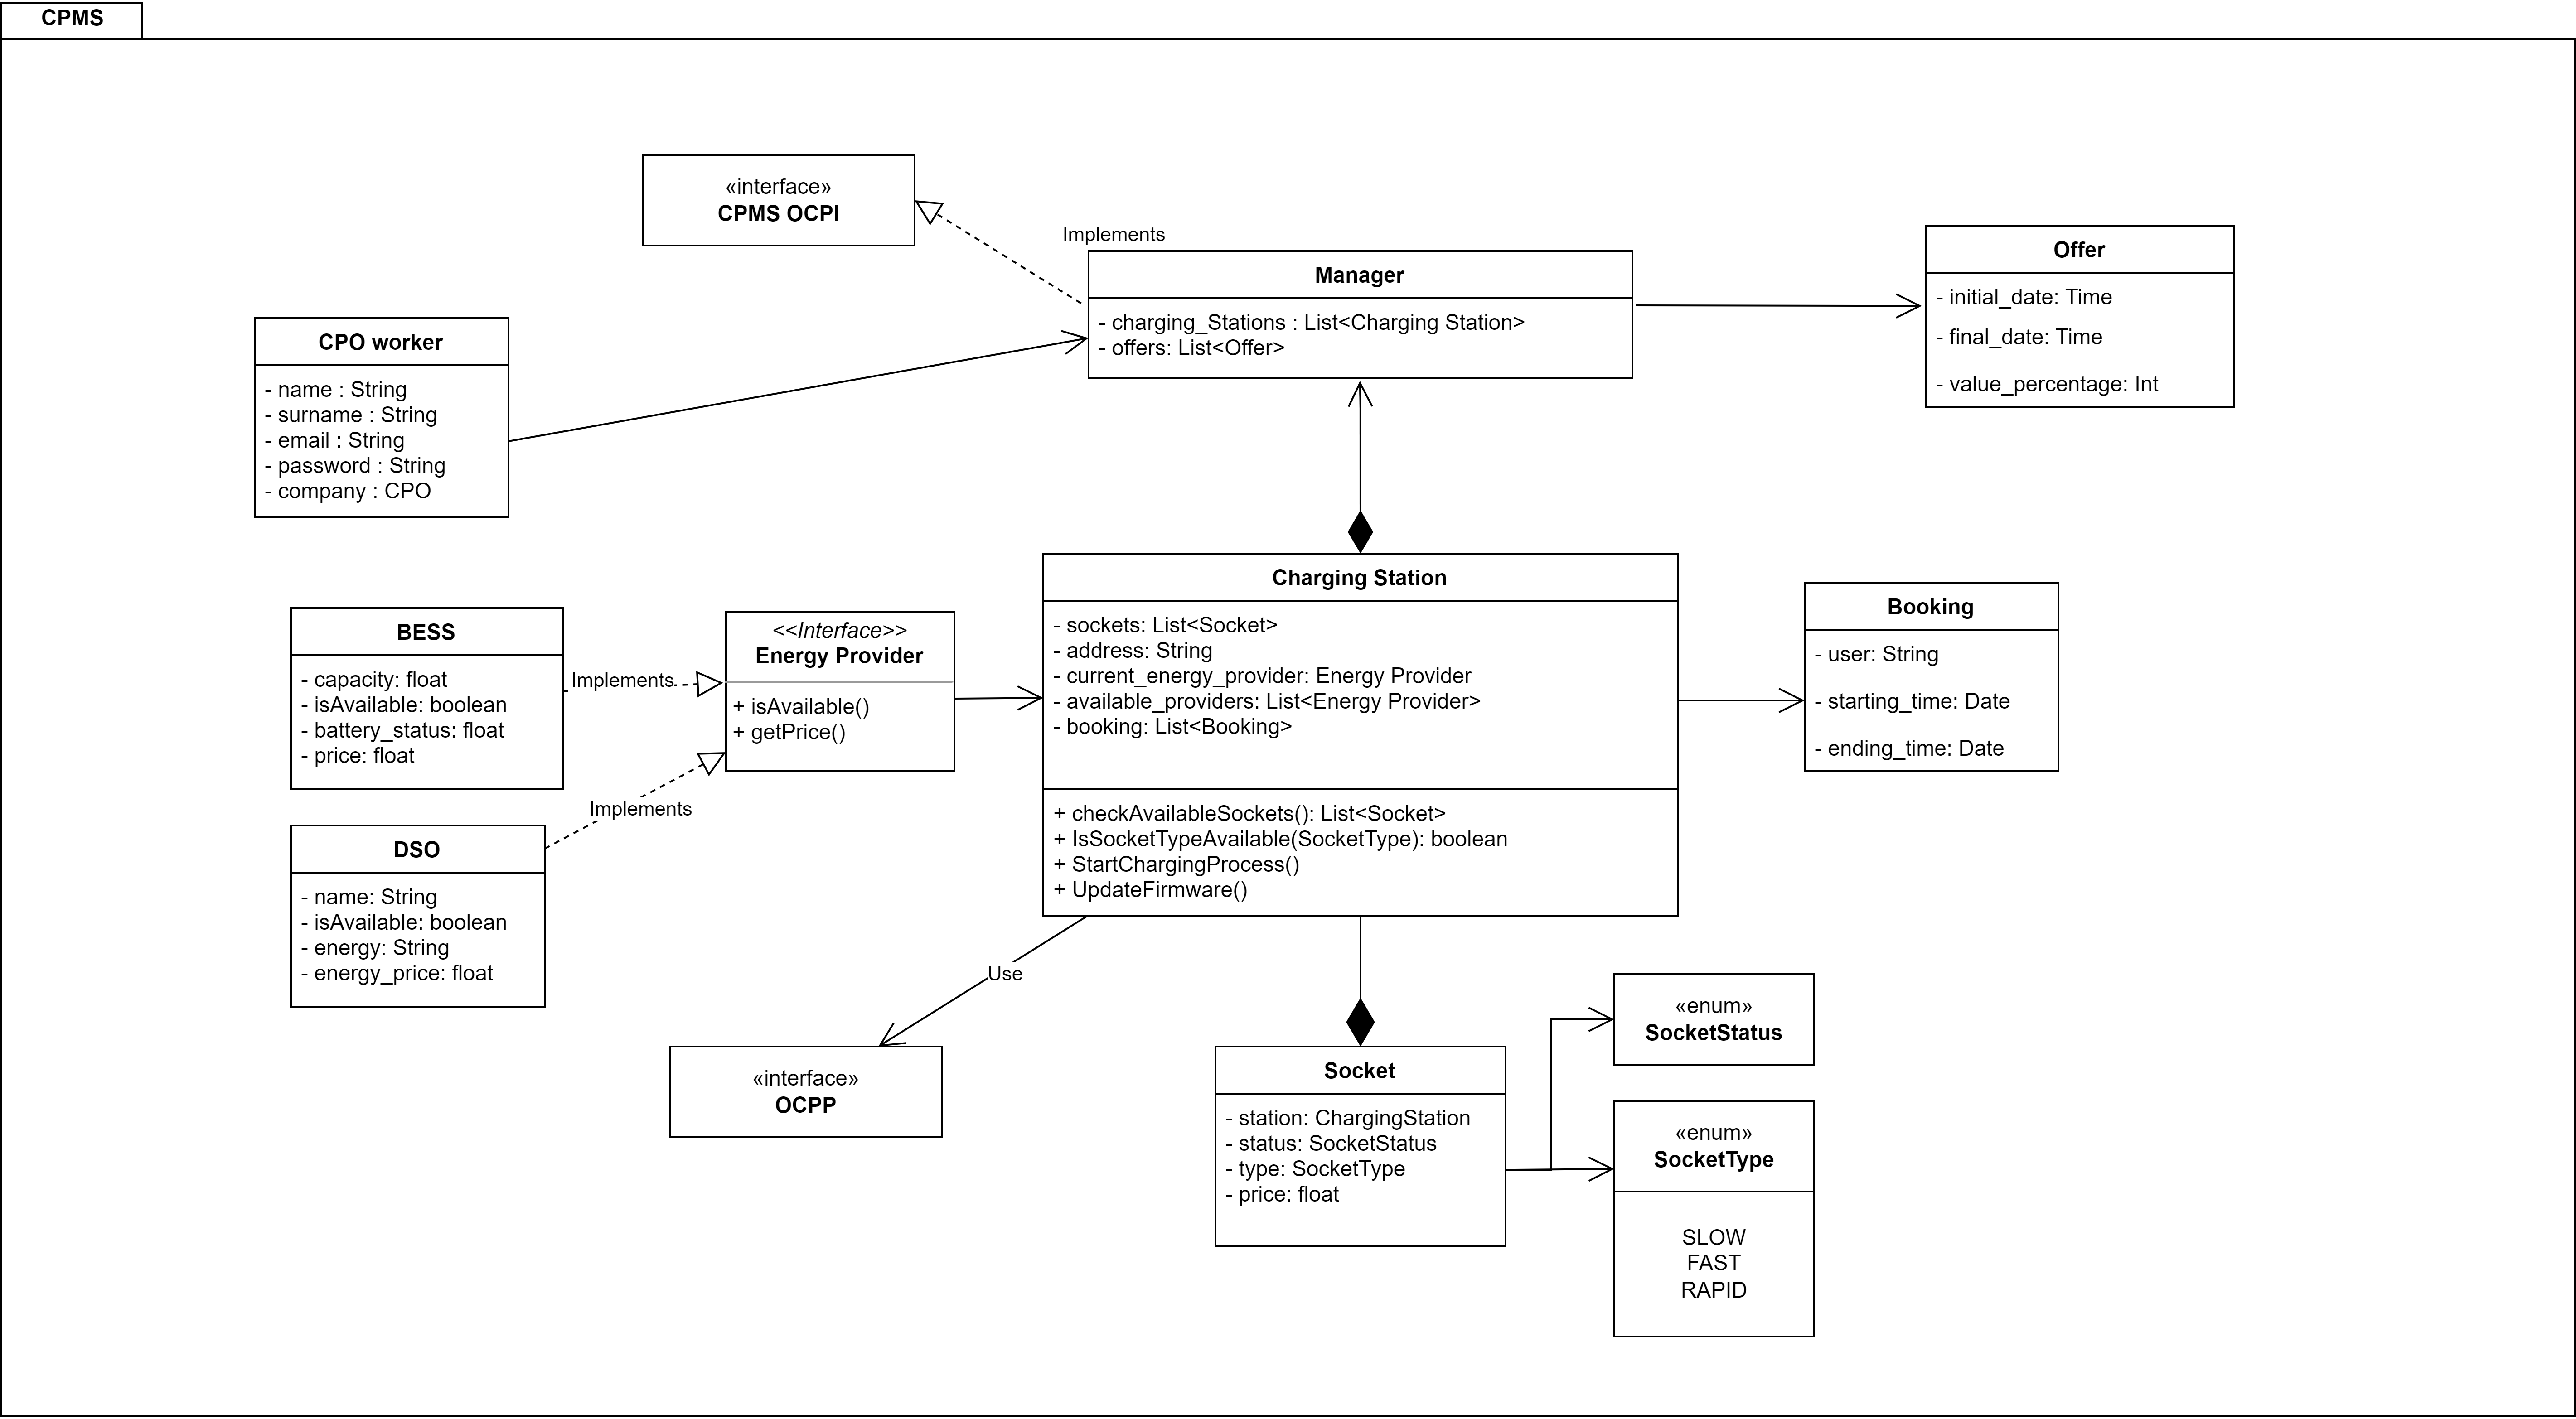
\includegraphics[scale=0.55, center]{assets/UML_CPMS.png}
                    \caption{High-level UML - CPMS Subsystem}
                    \label{fig: UML CPMS}
                \end{figure}
            \end{center}

    \newpage
    \subsection{Product functions}
    \label{product_functions}
    
        \subsubsection{Sign-up}
        \begin{itemize}
            \item \textbf{Sign-up:} let the user sign-up thorugh an email and a password.
        
            \begin{center}
                \begin{figure}[!h]
                    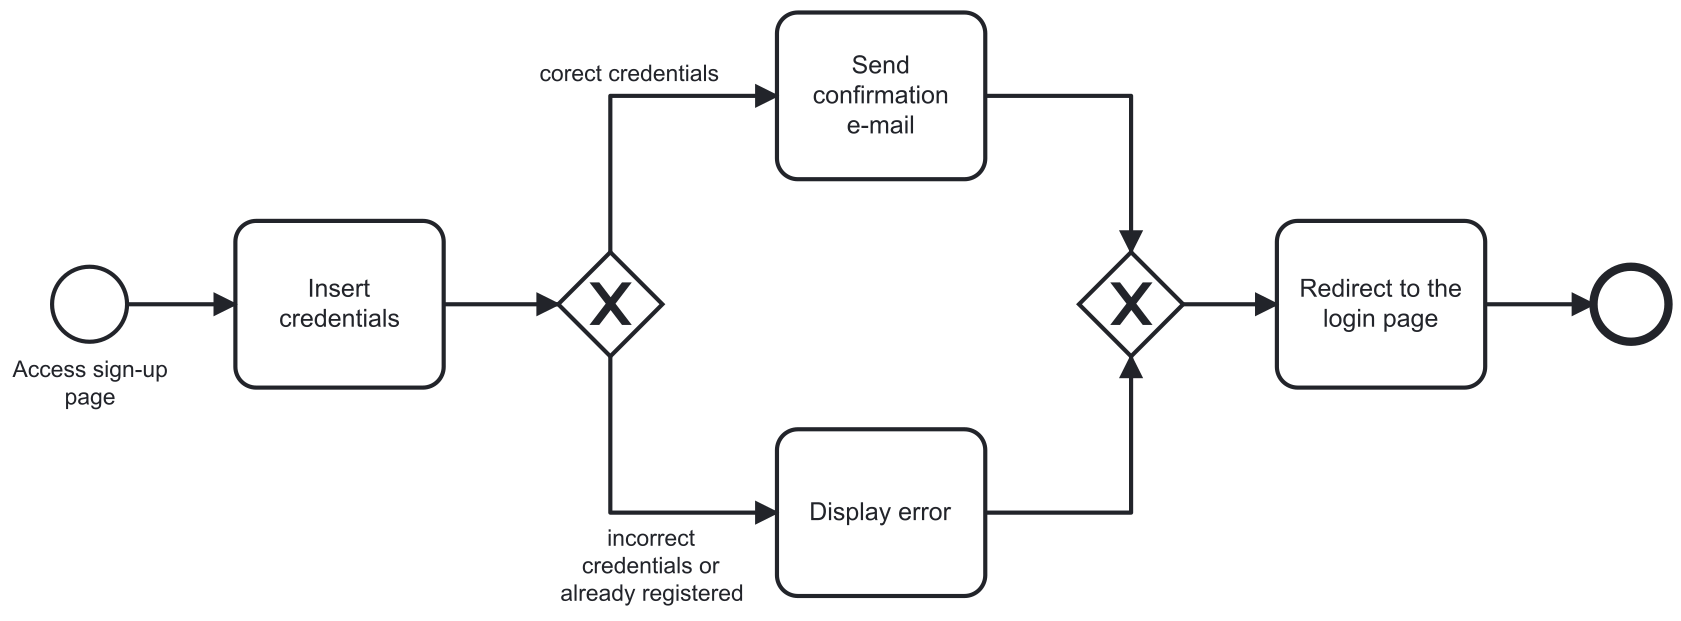
\includegraphics[width=\textwidth]{assets/bpmn/sign-up.png}
                    \caption{Sign Up BPMN}
                    \label{fig: singup}
                \end{figure}
            \end{center}
        \end{itemize}
        
        \newpage
        \subsubsection{Check nearby stations}
        \begin{itemize}                                 
            \item \textbf{Check aera:} let the user check the nearby charging stations through an inter map and the GPS position.
        
            \begin{center}
                \begin{figure}[!h]
                    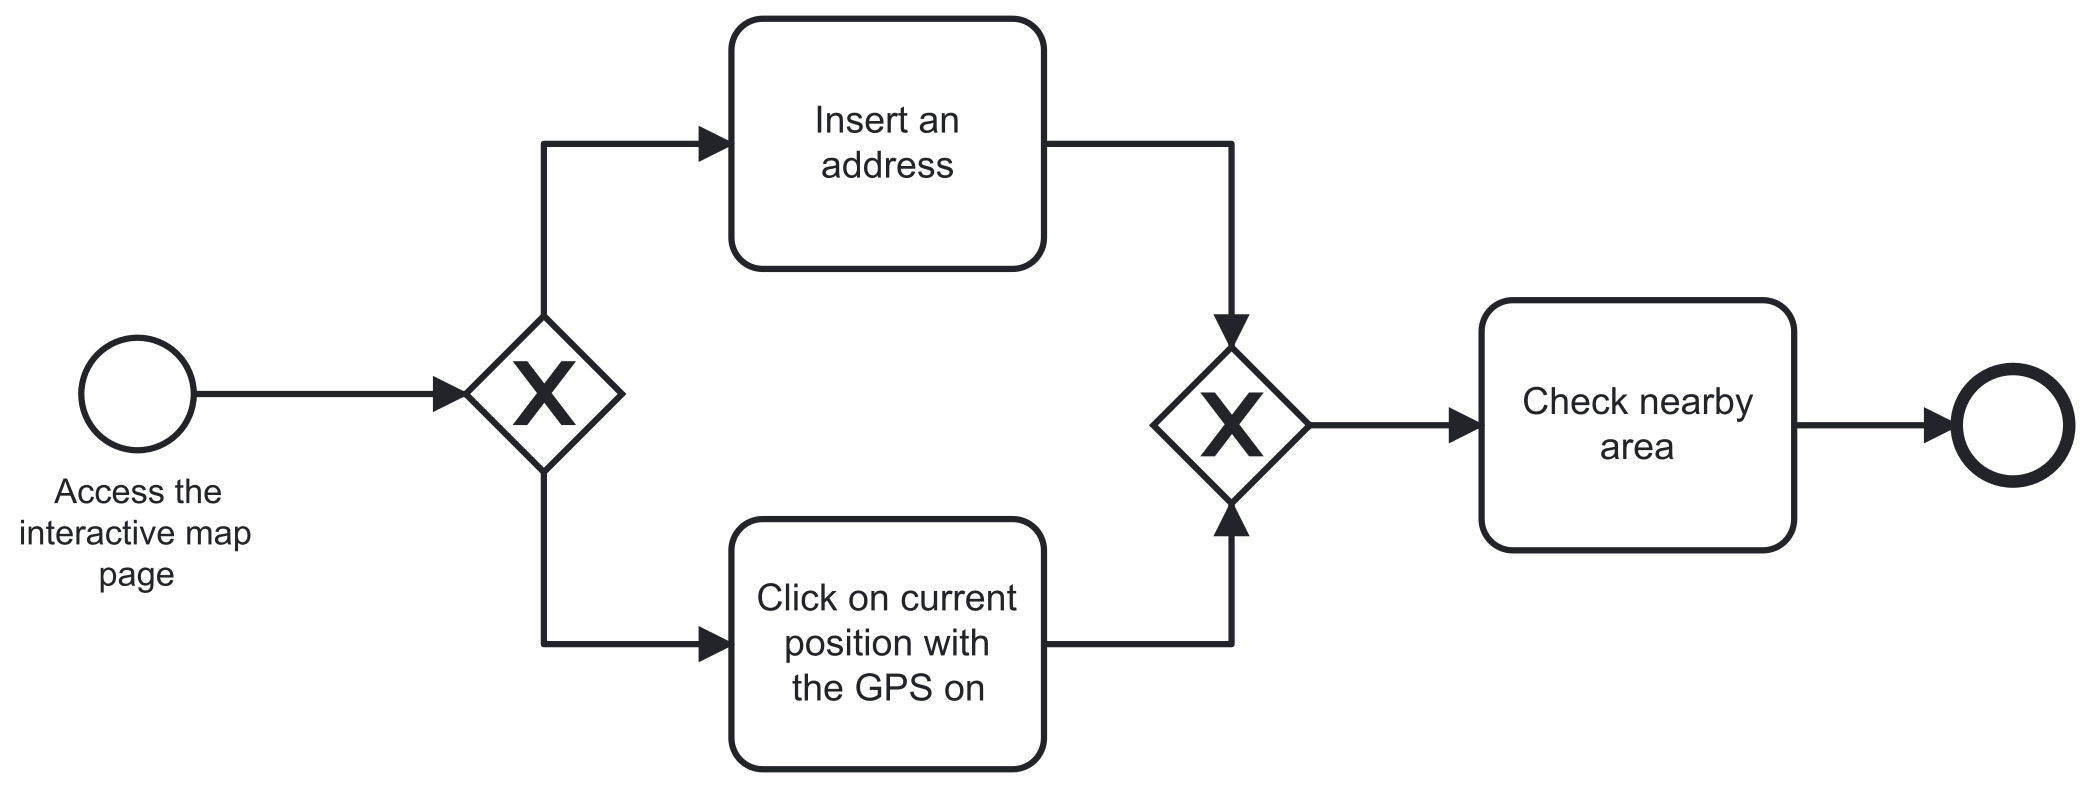
\includegraphics[scale=0.60, center]{assets/bpmn/Check area.png}
                    \caption{check nearby stations}
                    \label{fig: check nearby stations}
                \end{figure}
            \end{center}
        \end{itemize}
        
        
        \subsubsection{Smart suggestions}
        \begin{itemize}                                 
            \item \textbf{Suggestions:} notify the user about the best charging stations to use based on the user's schedule and the current price.
            
            \begin{center}
                \begin{figure}[!h]
                    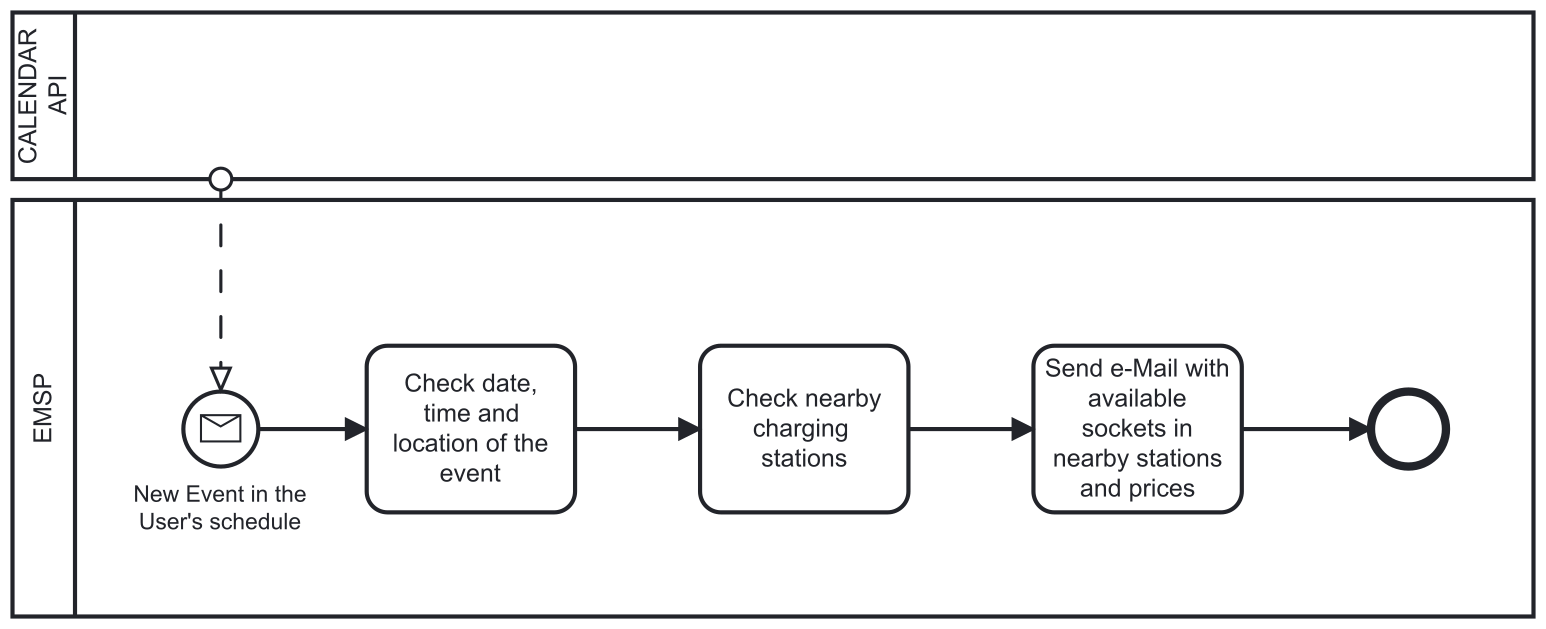
\includegraphics[scale=0.60, center]{assets/bpmn/Suggestions.png}
                    \caption{User's schedule suggestions}
                    \label{fig: User's schedule suggestions}
                \end{figure}
            \end{center}
        \end{itemize}

        \newpage
        \subsubsection{Booking a charging spot}
        \begin{itemize}                                 
            \item \textbf{Booking:} let the user book a charging spot for a specific timeframe. The user can also see the available charging spots and the price for each one.
            
            \begin{center}
                \begin{figure}[!h]
                    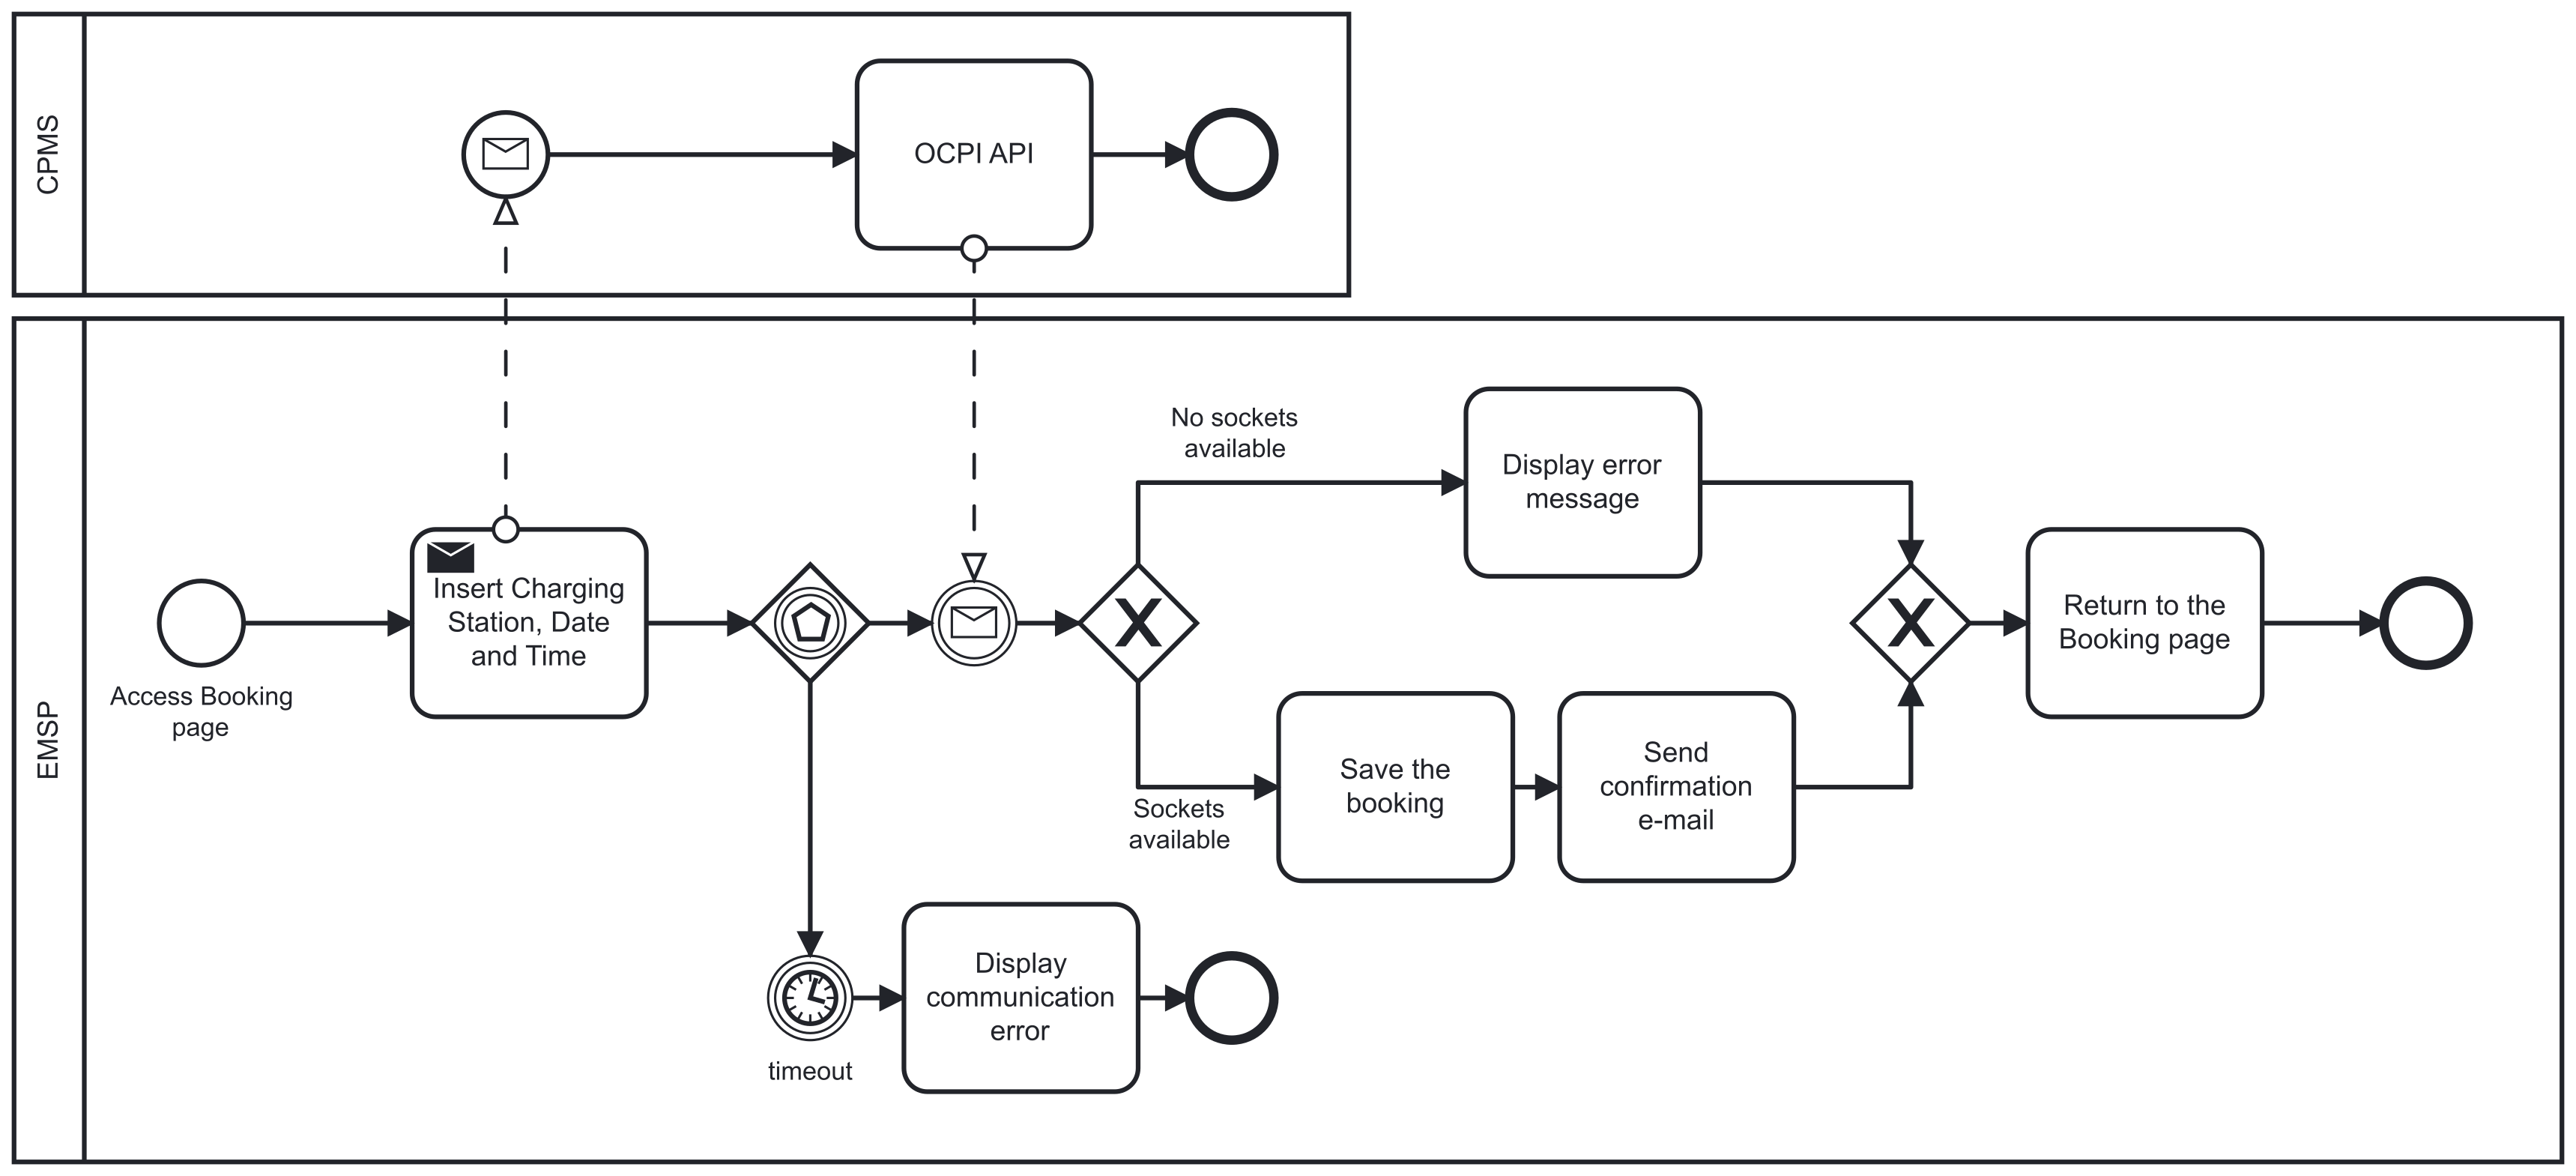
\includegraphics[width=\textwidth]{assets/bpmn/Booking.png}
                    \caption{Booking a charging spot}
                    \label{fig: Booking a charging spot}
                \end{figure}
            \end{center}
        \end{itemize}

        \newpage
        \subsubsection{Charging Process}
        \begin{itemize}                                 
            \item \textbf{Charging Process:} let the user start the charging process and pay for the service.
        
            \begin{center}
                \begin{figure}[!h]
                    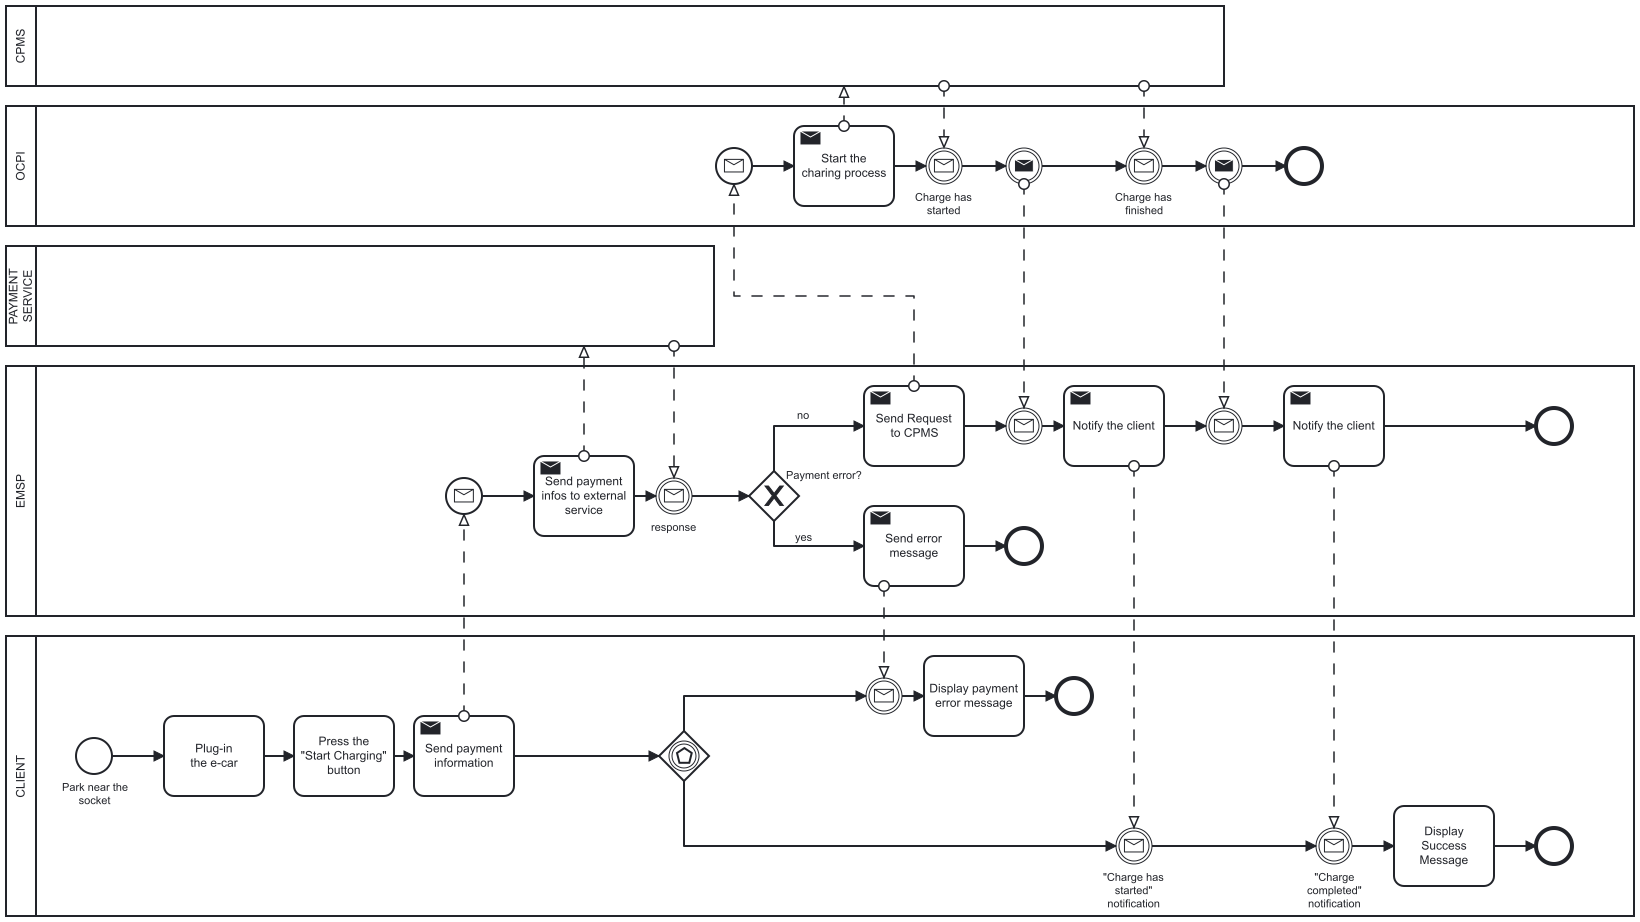
\includegraphics[width=\textwidth]{assets/bpmn/Charging Process.png}
                    \caption{Charging Process}
                    \label{fig: Charging Process}
                \end{figure}
            \end{center}
        \end{itemize}
        
    
    \newpage
    \subsection{User characteristics}
    The application has been thought for anybody that owns an electric car and wants to plan his charging process. 
    Because of this, the potential user base comprises of any electric vehicle owner with a device connected to the internet.
    The user should also be capable of interacting with a webapp
        
    \subsection{Assumptions, dependencies and constraints}
    \newcounter{assumptionCtr}
    \begin{itemize}
        \item \stepcounter{assumptionCtr}D\arabic{assumptionCtr}: Users have access to the internet while using the web application
        \item \stepcounter{assumptionCtr}D\arabic{assumptionCtr}: The infrastructure of the charging stations is reliable and works 99\% of the time
        \item \stepcounter{assumptionCtr}D\arabic{assumptionCtr}: User's car works properly while charging
        \item \stepcounter{assumptionCtr}D\arabic{assumptionCtr}: Information about the charging stations offered by the CPMS are accurate (such as position, state and availability )
        \item \stepcounter{assumptionCtr}D\arabic{assumptionCtr}: The DSO's infrastructure is working and their data is reliable 
        \item \stepcounter{assumptionCtr}D\arabic{assumptionCtr}: Information about the user's schedule is correct and meaningful
        \item \stepcounter{assumptionCtr}D\arabic{assumptionCtr}: Users own an IT device to connect to the application
        \item \stepcounter{assumptionCtr}D\arabic{assumptionCtr}: Each user registers only once, and always feeds correct information to the app     
        \item \stepcounter{assumptionCtr}D\arabic{assumptionCtr}: The data supplied by the user's devices are correct (battery charge, current position)
        \item \stepcounter{assumptionCtr}D\arabic{assumptionCtr}: Special offers regarding the charging stations are correct and reliable
        \item \stepcounter{assumptionCtr}D\arabic{assumptionCtr}: Special offers provided by one CPO concern all the charging stations owned by that CPO
        \item \stepcounter{assumptionCtr}D\arabic{assumptionCtr}: The eMSPs and all the connected CPMSs follow the OCPI 2.2.1 protocol
       \end{itemize}


    
    
    
    \newpage
    \section{Specific Requirements}
    
    \subsection{External Interface Requirements}

    \subsubsection{User Interfaces}
    Users should interface the web application through devices that must be connected to the Internet. The service will be accessed through a web browser from the web site domain (i.g. www.eMall.com).
    As the service will be used by a lot of different kinds of users, the web application interface should be as simple and intuitive as possible.
    

    \subsubsection{Hardware Interfaces}
    \label{hardware_interfaces}
    Since the system provides a web application, there's not an hardware interface. 
    In order to give a complete experience, the system should be given the access/permission to the user's GPS position or navigation system.  

    \subsubsection{Software Interfaces}
    \label{software_interfaces}
    To access the application a web browser is required. Additional software like a calendar and GPS is necessary for accessing all the funcionalities of the application. The software will also take advantage of some interfaces to accomplish its requirements. An external API is necessary to visualize on maps the user location and the near charging stations. %frase copiatissima%
    
    \subsubsection{Communication Interfaces}
    Internet connections will be mandatory since the web application must communicate with the web server and the CPMS APIs.
    Communication with the CPMS will be ASYNCRONOUS/etc..

    \newpage
    \subsection{Functional Requirements}

    \subsubsection{List of Requirements}
    \newcounter{RequirementCtr}
    \rowcolors{2}{}{PineGreen!25}
    \underline{Shared Requirements}
    \begin{longtable}{|c|p{0.69\textwidth}|}
        \hline
        \textbf{ID} & \textbf{Requirement}\\ \hline\hline
        \stepcounter{RequirementCtr}
        R\arabic{RequirementCtr}    & The system must allow registered and logged-in users to use the app.\\\hline
        \stepcounter{RequirementCtr}
        R\arabic{RequirementCtr}    & The system must respect the GDPR and the user's privacy.\\\hline
        \stepcounter{RequirementCtr}
        R\arabic{RequirementCtr}    & The system must allow registered users to log-in using their e-mail\\\hline
        \stepcounter{RequirementCtr}
        R\arabic{RequirementCtr}    & Both the CMPS and the eMSP subsystem must abide to the OCPI 2.2.1 protocol \\\hline
    \end{longtable}  
    \rowcolors{1}{white!100}{} 
    \rowcolors{2}{}{PineGreen!25}
    \underline{EMSP Subsystem Requirements}
    \begin{longtable}{|c|p{0.69\textwidth}|}
        \hline
        \textbf{ID} & \textbf{Requirement}\\ \hline\hline       
        \stepcounter{RequirementCtr}
        R\arabic{RequirementCtr}    & The eMSP subsystem must show the user the nearby charging stations through an interactive map.\\\hline  
        \stepcounter{RequirementCtr}
        R\arabic{RequirementCtr}    & The eMSP subsystem must be allowed to use the user's GPS location in order to view the nearby charging stations, if given permission.\\\hline  
        \stepcounter{RequirementCtr}
        R\arabic{RequirementCtr}    & The eMSP subsystem must notify the user when the charge has finished.\\\hline
        \stepcounter{RequirementCtr}
        R\arabic{RequirementCtr}    & The eMSP subsystem must noitify the user about discounted prices.\\\hline
        \stepcounter{RequirementCtr}
        R\arabic{RequirementCtr}    & The eMSP subsystem must show the user the prices of the charging stations.\\\hline
        \stepcounter{RequirementCtr}
        R\arabic{RequirementCtr}    & The eMSP subsystem must access the User calendar schedule in order to suggest the best charging timeframes, if given permission.\\\hline
        \stepcounter{RequirementCtr}
        R\arabic{RequirementCtr}    & The eMSP subsystem must suggest the user on which charging stations to go based on the car battery and his daily schedule.\\\hline
        \stepcounter{RequirementCtr}
        R\arabic{RequirementCtr}    & The eMSP subsystem must communicate with the CPMSs in order to retrieve all needed information about the charging stations.\\\hline
        \stepcounter{RequirementCtr}
        R\arabic{RequirementCtr}    & The eMSP subsystem must allow the user to book a charging spot for a future date.\\\hline
        \stepcounter{RequirementCtr}
        R\arabic{RequirementCtr}    & The eMSP subsystem must allow the user to cancel a future reservation for a charging spot.\\\hline
        \stepcounter{RequirementCtr}
        R\arabic{RequirementCtr}    & The eMSP subsystem must allow the user to pay for the charge through an external payment service.\\\hline
        \stepcounter{RequirementCtr}
        R\arabic{RequirementCtr}    & The eMSP subsystem must allow the user to start or stop the charge via the application.\\\hline
        \stepcounter{RequirementCtr}
        R\arabic{RequirementCtr}    & The eMSP subsystem must notify the user of the upcoming booked sessions.\\\hline
    \end{longtable}  
    \rowcolors{1}{white!100}{}  
    \rowcolors{2}{}{PineGreen!25}
    \underline{CPMS Subsystem Requirements}
    \begin{longtable}{|c|p{0.69\textwidth}|}
        \hline
        \textbf{ID} & \textbf{Requirement}\\ \hline\hline
        \stepcounter{RequirementCtr}
        R\arabic{RequirementCtr}    & The CPMS subsystem must communicate with the DSO according to a standard protocol.\\\hline
        \stepcounter{RequirementCtr}
        R\arabic{RequirementCtr}    & The CPMS subsystem must retrieve the DSO current energy price.\\\hline
        \stepcounter{RequirementCtr}
        R\arabic{RequirementCtr}    & The CPMS subsystem must automatically decide from which DSO to acquire energy.\\\hline
        \stepcounter{RequirementCtr}
        R\arabic{RequirementCtr}    & The CPMS subsystem must retrieve the charging station's battery status.\\\hline
        \stepcounter{RequirementCtr}
        R\arabic{RequirementCtr}    & The CPMS subsystem must dynamically change the energy source depending on the internal station's battery status and the available DSOs' prices.\\\hline
        \stepcounter{RequirementCtr}
        R\arabic{RequirementCtr}    & The CPMS subsystem must communicate the location of the charging stations to all connected eMSPs.\\\hline
        \stepcounter{RequirementCtr}
        R\arabic{RequirementCtr}    & The CPMS subsystem must retrieve the internal status of the sockets through the OCPP standard protocol.\\\hline
        \stepcounter{RequirementCtr}
        R\arabic{RequirementCtr}    & The CPMS subsystem must retrieve and communicate to all connected eMSPs the external status of the sockets through the OCPI standard protocol.\\\hline
        \stepcounter{RequirementCtr}
        R\arabic{RequirementCtr}    & The CPMS subsystem must allow to start or stop a charging session through the OCPP standard protocol.\\\hline
        \stepcounter{RequirementCtr}
        R\arabic{RequirementCtr}    & The CPMS subsystem must retrieve the battery status of the car through the DIN/ISO specifications.\\\hline
        \stepcounter{RequirementCtr}
        R\arabic{RequirementCtr}    & The CPMS subsystem must allow the CPOW to change the price of a charging station.\\\hline
        \stepcounter{RequirementCtr}
        R\arabic{RequirementCtr}    & The CPMS subsystem must allow the CPOW to add or change the current special offer.\\\hline
        \stepcounter{RequirementCtr}
        R\arabic{RequirementCtr}    & The CPMS subsystem must allow the CPOW to change the energy provider of a charging station.\\\hline
        \stepcounter{RequirementCtr}
        R\arabic{RequirementCtr}    & The CPMS subsystem must unlock the reserved charging spot if the user doesn't show up.\\\hline

    \end{longtable}

    \subsubsection{Mapping}
    \rowcolors{1}{white!100}{}
    \newcounter{goalCtr2}
    %written explanation of how the G,D and R go together

    \underline{User Goals}
    \begin{table}[H]
        \begin{center}
            \begin{tabular}{|c | p{0.69\textwidth}|}
                \hline
                \cellcolor{blue!30}\textbf{\stepcounter{goalCtr2}G\arabic{goalCtr2}} &  Know about the charging stations nearby, including their cost and any special offer they have.\\\hline
                \cellcolor{pink!50}R1 & Text.\\\hline
                \cellcolor{pink!50}R2 & Text.\\\hline
                \cellcolor{pink!50}R3 & Text.\\\hline 
                \cellcolor{pink!50}R5 & The eMSP subsystem must show the user the nearby charging stations through an interactive map.\\\hline
                \cellcolor{pink!50}R6 & The eMSP subsystem must be allowed to use the user's GPS location in order to view the nearby charging stations, if given permission.\\\hline
                \cellcolor{pink!50}R8 & The eMSP subsystem must noitify the user about discounted prices.\\\hline
                \cellcolor{pink!50}R9 & The eMSP subsystem must show the user the prices of the charging stations.\\\hline
                \cellcolor{green!50}D & .\\\hline
            \end{tabular}
        \end{center}
    \end{table}

    \begin{table}[H]
        \begin{center}
            \begin{tabular}{|c | p{0.69\textwidth}|}
                \hline
                \cellcolor{blue!30}\textbf{\stepcounter{goalCtr2}G\arabic{goalCtr2}} & Book a charge in a specific charging station for a certain timeframe.\\\hline
                \cellcolor{pink!50}R1 &  Text.\\\hline
                \cellcolor{pink!50}R2 &  Text.\\\hline
                \cellcolor{pink!50}R3 &  Text.\\\hline
                \cellcolor{pink!50}R13 & TEXT\\\hline
                \cellcolor{pink!50}R14 & TEXT\\\hline
                \cellcolor{pink!50}R17 & TEXT\\\hline
                \cellcolor{pink!50}R31 & TEXT\\\hline
                \cellcolor{green!50}D & .\\\hline
            \end{tabular}
        \end{center}
    \end{table}

    \begin{table}[H]
        \begin{center}
            \begin{tabular}{|c | p{0.69\textwidth}|}
                \hline
                \cellcolor{blue!30}\textbf{\stepcounter{goalCtr2}G\arabic{goalCtr2}} & Start the charging process at a certain station.\\\hline
                \cellcolor{pink!50}R1 &  Text.\\\hline
                \cellcolor{pink!50}R2 &  Text.\\\hline
                \cellcolor{pink!50}R3 &   Text.\\\hline
                \cellcolor{pink!50}R4 & TEXT\\\hline
                \cellcolor{pink!50}R7 & TEXT\\\hline
                \cellcolor{pink!50}R16 & TEXT\\\hline
                \cellcolor{pink!50}R26 & TEXT\\\hline
                \cellcolor{green!50}D & .\\\hline
            \end{tabular}
        \end{center}
    \end{table}

    \begin{table}[H]
        \begin{center}
            \begin{tabular}{|c | p{0.69\textwidth}|}
                \hline
                \cellcolor{blue!30}\textbf{\stepcounter{goalCtr2}G\arabic{goalCtr2}} & Pay for the obtained service.\\\hline
                \cellcolor{pink!50}R1 &  Text.\\\hline
                \cellcolor{pink!50}R2 &  Text.\\\hline
                \cellcolor{pink!50}R3 &   Text.\\\hline
                \cellcolor{pink!50}R15 & TEXT\\\hline
                \cellcolor{green!50}D & .\\\hline
            \end{tabular}
        \end{center}
    \end{table}

    \underline{eMSP Subsystem Goals}
    \begin{table}[H]
        \begin{center}
            \begin{tabular}{|c | p{0.69\textwidth}|}
                \hline
                \cellcolor{blue!30}\textbf{\stepcounter{goalCtr2}G\arabic{goalCtr2}} & Be able to communicate with multiple CPMS.\\\hline
                \cellcolor{pink!50}R4 & TEXT\\\hline
                \cellcolor{green!50}D & .\\\hline
            \end{tabular}
        \end{center}
    \end{table}

    \begin{table}[H]
        \begin{center}
            \begin{tabular}{|c | p{0.69\textwidth}|}
                \hline
                \cellcolor{blue!30}\textbf{\stepcounter{goalCtr2}G\arabic{goalCtr2}} & Suggest the user convenient charging timeframes based on his upcoming schedule.\\\hline
                \cellcolor{pink!50}R10 & TEXT\\\hline
                \cellcolor{pink!50}R11 & TEXT\\\hline
                \cellcolor{green!50}D & .\\\hline
            \end{tabular}
        \end{center}
    \end{table}

    \begin{table}[H]
        \begin{center}
            \begin{tabular}{|c | p{0.69\textwidth}|}
                \hline
                \cellcolor{blue!30}\textbf{\stepcounter{goalCtr2}G\arabic{goalCtr2}} & Notify the user when the charging process is finished.\\\hline
                \cellcolor{pink!50}R7 & TEXT\\\hline
                \cellcolor{green!50}D & .\\\hline
            \end{tabular}
        \end{center}
    \end{table}

    \begin{table}[H]
        \begin{center}
            \begin{tabular}{|c | p{0.69\textwidth}|}
                \hline
                \cellcolor{blue!30}\textbf{\stepcounter{goalCtr2}G\arabic{goalCtr2}} & Be able to communicate with multiple eMSPs.\\\hline
                \cellcolor{pink!50}R4 & TEXT\\\hline
                \cellcolor{pink!50}R23 & TEXT\\\hline
                \cellcolor{pink!50}R25 & TEXT\\\hline
                \cellcolor{green!50}D & .\\\hline
            \end{tabular}
        \end{center}
    \end{table}
   
    \begin{table}[H]
        \begin{center}
            \begin{tabular}{|c | p{0.69\textwidth}|}
                \hline
                \cellcolor{blue!30}\textbf{\stepcounter{goalCtr2}G\arabic{goalCtr2}} & Be able to communicate with at least one DSO.\\\hline
                \cellcolor{pink!50}R18 & TEXT\\\hline
                \cellcolor{green!50}D & .\\\hline
            \end{tabular}
        \end{center}
    \end{table}

    \begin{table}[H]
        \begin{center}
            \begin{tabular}{|c | p{0.69\textwidth}|}
                \hline
                \cellcolor{blue!30}\textbf{\stepcounter{goalCtr2}G\arabic{goalCtr2}} & Communicate the location and the "external" status of the charging station.\\\hline
                \cellcolor{pink!50}R23 & TEXT\\\hline
                \cellcolor{pink!50}R25 & TEXT\\\hline
                \cellcolor{green!50}D & .\\\hline
            \end{tabular}
        \end{center}
    \end{table}

    \begin{table}[H]
        \begin{center}
            \begin{tabular}{|c | p{0.69\textwidth}|}
                \hline
                \cellcolor{blue!30}\textbf{\stepcounter{goalCtr2}G\arabic{goalCtr2}} & Know the internal status of a charging station.\\\hline
                \cellcolor{pink!50}R21 & TEXT\\\hline
                \cellcolor{pink!50}R24 & TEXT\\\hline
                \cellcolor{green!50}D & .\\\hline
            \end{tabular}
        \end{center}
    \end{table}

    \begin{table}[H]
        \begin{center}
            \begin{tabular}{|c | p{0.69\textwidth}|}
                \hline
                \cellcolor{blue!30}\textbf{\stepcounter{goalCtr2}G\arabic{goalCtr2}} & Start charging a vehicle according to the amount of power supplied by the socket, and monitor the charging process to infer when the battery is full.\\\hline
                \cellcolor{pink!50}R26 & TEXT\\\hline
                \cellcolor{pink!50}R27 & TEXT\\\hline
                \cellcolor{green!50}D & .\\\hline
            \end{tabular}
        \end{center}
    \end{table}

    \begin{table}[H]
        \begin{center}
            \begin{tabular}{|c | p{0.69\textwidth}|}
                \hline
                \cellcolor{blue!30}\textbf{\stepcounter{goalCtr2}G\arabic{goalCtr2}} & Acquire from the DSOs information about the current price of energy.\\\hline
                \cellcolor{pink!50}R19 & TEXT\\\hline
                \cellcolor{green!50}D & .\\\hline
            \end{tabular}
        \end{center}
    \end{table}

    \begin{table}[H]
        \begin{center}
            \begin{tabular}{|c | p{0.69\textwidth}|}
                \hline
                \cellcolor{blue!30}\textbf{\stepcounter{goalCtr2}G\arabic{goalCtr2}} & Decide from which DSO to acquire energy (if more than one is available).\\\hline
                \cellcolor{pink!50}R20 & TEXT\\\hline
                \cellcolor{pink!50}R22 & TEXT\\\hline
                \cellcolor{pink!50}R30 & TEXT\\\hline
                \cellcolor{green!50}D & .\\\hline
            \end{tabular}
        \end{center}
    \end{table}

    \begin{table}[H]
        \begin{center}
            \begin{tabular}{|c | p{0.69\textwidth}|}
                \hline
                \cellcolor{blue!30}\textbf{\stepcounter{goalCtr2}G\arabic{goalCtr2}} & Dynamically decide where to get energy for charging (station battery, DSO, or a mix according to availability and cost).\\\hline
                \cellcolor{pink!50}R21 & TEXT\\\hline
                \cellcolor{pink!50}R22 & TEXT\\\hline
                \cellcolor{pink!50}R30 & TEXT\\\hline
                \cellcolor{green!50}D & .\\\hline
            \end{tabular}
        \end{center}
    \end{table}

    \underline {CPOW goals}
    \begin{table}[H]
        \begin{center}
            \begin{tabular}{|c | p{0.69\textwidth}|}
                \hline
                \cellcolor{blue!30}\textbf{\stepcounter{goalCtr2}G\arabic{goalCtr2}} & Change the source of energy between batteries and grid.\\\hline
                \cellcolor{pink!50}R1 &  Text.\\\hline
                \cellcolor{pink!50}R2 &  Text.\\\hline
                \cellcolor{pink!50}R3 &   Text.\\\hline
                \cellcolor{pink!50}R30 & TEXT\\\hline
                \cellcolor{green!50}D & .\\\hline
            \end{tabular}
        \end{center}
    \end{table}

    \begin{table}[H]
        \begin{center}
            \begin{tabular}{|c | p{0.69\textwidth}|}
                \hline 
                \cellcolor{blue!30}\textbf{\stepcounter{goalCtr2}G\arabic{goalCtr2}} & Insert special and limited owners.\\\hline
                \cellcolor{pink!50}R1 &  Text.\\\hline
                \cellcolor{pink!50}R2 &  Text.\\\hline
                \cellcolor{pink!50}R3 &  Text.\\\hline
                \cellcolor{pink!50}R29 & TEXT\\\hline
                \cellcolor{green!50}D & .\\\hline
            \end{tabular}
        \end{center}
    \end{table}

    \begin{table}[H]
        \begin{center}
            \begin{tabular}{|c | p{0.69\textwidth}|}
                \hline
                \cellcolor{blue!30}\textbf{\stepcounter{goalCtr2}G\arabic{goalCtr2}} & Change the price of a charging station.\\\hline
                \cellcolor{pink!50}R1 &  Text.\\\hline
                \cellcolor{pink!50}R2 &  Text.\\\hline
                \cellcolor{pink!50}R3 &   Text.\\\hline
                \cellcolor{pink!50}R28 & TEXT\\\hline
                \cellcolor{green!50}D & .\\\hline
            \end{tabular}
        \end{center}
    \end{table}

    \newpage
    \subsubsection{Use Cases}
    \setcounter{secnumdepth}{4}

    \paragraph{Use Cases Diagram}
    \begin{itemize}
        \item \textbf {Policy Makers}
        \begin{center}
            \begin{figure}[H]
                
\includegraphics[scale=0.55, center]{assets/placeholder.png}
                \caption{Policy Maker - Use Case Diagram}
                \label{fig: UseCase_PolicyMaker}
            \end{figure}
        \end{center}
        \newpage
        \item \textbf {Farmers}
        \begin{center}
            \begin{figure}[H]
                
\includegraphics[scale=0.60, center]{assets/placeholder.png}
                \caption{Farmer - Use Case Diagram}
                \label{fig: UseCase_Farmer}
            \end{figure}
        \end{center}
        \newpage
        \item \textbf {Agronomists}
        \begin{center}
            \begin{figure}[H]
                
\includegraphics[scale=0.60, center]{assets/placeholder.png}
                \caption{Agronomist - Use Case Diagram}
                \label{fig: UseCase_Agronomist}
            \end{figure}
        \end{center}
        \newpage
    \end{itemize}

    \paragraph{Use Cases Description}

    For more details \ref{sequencediagram}.
    
        \begin{itemize}
            \item \textbf {Shared Use Cases}
            
            \begin{table}[H]
                \item[] \textbf{Sign Up}
                \item[] 
                \centering
                \begin{tabular}{|c |m{0.69\textwidth}|}
                    \hline
                    \textbf{Use Case} & Sign Up\\ \hline
                    \textbf{Actor} & U\\ \hline
                    \textbf{Entry condition} & User wants to register in the system\\  \hline
                    \textbf{Flow of events} & \begin{enumerate}
                                                \item text
                                                
                                            \end{enumerate}\\ \hline
                    \textbf{Exit condition} & User data are saved into the system and registration ends successfully  \\ \hline
                    \textbf{Exceptions} &  \begin{enumerate}
                        \item text
                        
                    \end{enumerate}
                    An error message is shown and the flow of events starts again from point 3\\ \hline                    
                \end{tabular}
            \end{table}

           
            \item \textbf {U}


            \newpage
            \item \textbf{text}
            
           


        \item \textbf{Use Cases to requirement mapping}
        0
        \item[] \begin{longtable}{|p{0.31\textwidth}|p{0.69\textwidth}|}
                    \hline
                    \cellcolor{SpringGreen!50}\textbf{1)Sign Up}\centering & R3) text
                                                                     
                                                                     R2) text\\\hline
                   
            \end{longtable}
    
    \end{itemize}

        \newpage
        \subsubsection{Sequence Diagrams} \label{sequencediagram} 
        \begin{itemize}
            \item \textbf{Shared Sequence Diagrams}\\
            
            \textbf{Sign Up}
            \begin{center}
                \begin{figure}[H]
                    
\includegraphics[scale=0.55, center]{assets/placeholder.png}
                    \caption{Shared Sequence Diagram - Sign Up Sequence Diagram}
                    \label{fig: sequence_signup}
                \end{figure}
            \end{center}

            \item \textbf{Farmers}\\

           
        \end{itemize}
        \newpage


    \subsection{Performance Requirements}
    text
    \subsection{Design Constraints}

    \subsubsection{Standards compliance}
    text
    %\subsubsection{Any other constraint}

    \subsection{Software System Attributes}
    \subsubsection{Reliability}
    text

    \subsubsection{Availability}
    text

    

    \begin{table}[H]
        \begin{center}
        \label{tab:availability}
        \begin{tabular}{l|c|r}
            \textbf{Component} & \textbf{Availability} & \textbf{Downtime}\\
            \hline
            cell here & cell here & cell here\\
            
            \hline
            cell here & cell here & cell here
        \end{tabular}
        \end{center}
    \end{table}

    \subsubsection{Security}
    %text here%
    \subsubsection{Maintainability}
    %text here%
    \subsubsection{Portability}
    %text here%
    \newpage
    \section{Formal Analysis using Alloy}
    \subsection{Formal Analysis Purpose}
    The following analysis aims to formally prove the correctness of the system model by exploiting Alloy verification tool. To achieve so, we test the model by checking if some of the previous defined goals are met. 

    Specifically, we stress:
    \begin{itemize}
        \item \textbf{(G3) }: 
        
    \end{itemize}

    Plus, we runned some empty predicates \texttt{show} to generate some more general instances of the app system.

    \end{document} % This is the end of the document